\section{顺序求解}
\label{sec:bo-sequential}

有了代理和采集函数，本节把它们接成一个完整的循环，回答一个具体问题：在预算$T$内，每一轮应当按什么次序做哪些计算，新读数又怎样改变下一轮的决策。

\paragraph{主要思想}
循环由两层组成，见图~\ref{fig:bo-loop}。外层是昂贵的真实评价，内层是便宜的计算：用数据建模，把模型转成分数，求分数的最大点。如果外层一次要几小时，内层花几秒钟算一个好的选点就很划算。

\begin{BookInlineFigure}
 \centering
 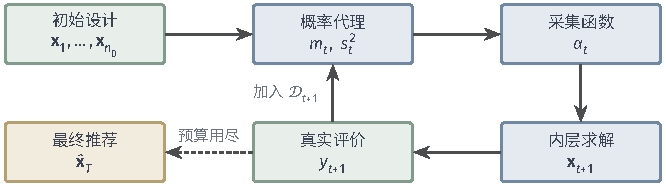
\includegraphics[width=112mm]{figures/05-optimization/05-stochastic-optimization/tikz/bo-loop/figure.pdf}
 \caption{贝叶斯优化的循环。绿框是需要运行真实目标的步骤，蓝框是只涉及代理模型的便宜计算，黄框是最后的输出。每轮读数加入$\mathcal{D}_{t+1}$，再回到概率代理更新。}
 \label{fig:bo-loop}
\end{BookInlineFigure}

每轮不必从头重算。第~\ref{sec:bo-posterior}节的后验本身是一个高斯过程，下一个读数相对它只是\emph{一个}新观测，把定理~\ref{thm:bo-posterior}应用于“以$(m_t,c_t)$为先验、只含一个观测”的情形，就得到更新式。记$\bm{x}^+=\bm{x}_{t+1}$，$y^+=y_{t+1}$，$v=s_t^2(\bm{x}^+)+\tau^2$，则
\begin{align}
 m_{t+1}(\bm{x})&=m_t(\bm{x})+\frac{c_t(\bm{x},\bm{x}^+)}{v}\bigl(y^+-m_t(\bm{x}^+)\bigr),
 \label{eq:bo-update-mean}\\
 c_{t+1}(\bm{x},\bm{x}')&=c_t(\bm{x},\bm{x}')-\frac{c_t(\bm{x},\bm{x}^+)\,c_t(\bm{x}',\bm{x}^+)}{v}.
 \label{eq:bo-update-cov}
\end{align}
式~\eqref{eq:bo-update-mean}说的是：新读数比预期低多少，其他位置就按它们与$\bm{x}^+$的后验协方差跟着调整多少，协方差为负的位置朝反方向调整。

\needspace{6\baselineskip}
\paragraph{变量}
贯穿例采用整数候选集，也就是把内层问题放在九个点上求解（内层的其他做法见第~\ref{sec:bo-inner}节）。计算中用到的量如下：
\begin{itemize}
 \item 已评价的位置与读数，长度为$t$的向量；
 \item 各候选点的后验均值$m_t$和后验协方差$c_t$，大小为$N\times N$，其中$N=9$；
 \item 当前最好值$b_t$；
 \item 每个候选点的采集分数，这里用EI。
\end{itemize}

\paragraph{初始化}
选取分散的初始点，运行真实评价，用定理~\ref{thm:bo-posterior}计算后验。例中初始点是$x=1,4,7$，读数$0.2,0.7,-0.3$，后验均值和标准差列在表~\ref{tab:bo-acq-values}中，$t=3$，$b_3=-0.3$。

\needspace{6\baselineskip}
\paragraph{每轮更新}
当$t<T$时，重复下面的步骤。
\begin{enumerate}
 \item \emph{计算采集分数。}对每个候选点按式~\eqref{eq:bo-ei}计算$\mathrm{EI}_t$。

 例中第一轮的分数见表~\ref{tab:bo-acq-values}，最大值$0.276$在$x=8$。

 \item \emph{选点并真实评价。}取分数最大的候选$\bm{x}^+$，运行目标，得到读数$y^+$。

 例中第一轮读到$f(8)=0.8$，比预期的$-0.151$高出很多，预测残差为
 \[
  y^+-m_3(8)\approx0.951.
 \]

 \item \emph{更新后验。}由式~\eqref{eq:bo-update-mean}和式~\eqref{eq:bo-update-cov}更新各候选点的均值和协方差，并更新$b_t$。

 例中$v=s_3^2(8)\approx0.750$，$c_3(6,8)\approx-0.187$，于是
 \[
  m_4(6)\approx-0.107+\frac{-0.187}{0.750}\times0.951\approx-0.345,
 \]
 \[
  s_4^2(6)\approx0.746-\frac{0.187^2}{0.750}\approx0.699.
 \]
 $x=6$的后验均值下降了，一次差的读数让另一个位置更有希望。由于$b_4$仍为$-0.3$，$\mathrm{EI}_4(6)$由$0.257$升到$0.356$，第二轮选$x=6$。
\end{enumerate}

$c_3(6,8)$的负号现在可以解释了。$x=6$和$x=8$都与$x=7$相关，而$F(7)$已知等于$-0.3$。在这个条件下，若$F(8)$比预期高，函数在$x=7$附近向右上升，光滑性要求它向左下降才能经过$F(7)$，于是$F(6)$偏低。

第二轮读到$f(6)=-1.0$，预测残差为$-0.655$，$v\approx0.699$，当前最好值变为$b_5=-1.0$。$x=5$与$x=6$的后验协方差$c_4(5,6)\approx0.431$，于是
\[
 m_5(5)\approx0.295+\frac{0.431}{0.699}\times(-0.655)\approx-0.109,
\]
\[
 s_5^2(5)\approx0.745-\frac{0.431^2}{0.699}\approx0.480.
\]

第三轮的分数变了样：$b_5$大幅降低，所有候选的EI都缩小了，
\[
 \mathrm{EI}_5(0)\approx0.042,\quad\mathrm{EI}_5(2)\approx0.037,\quad
 \mathrm{EI}_5(3)\approx0.020,\quad\mathrm{EI}_5(5)\approx0.032.
\]
EI选择了$x=0$，读到$f(0)=0.9$。此时$t=6=T$，预算用尽，循环结束。

最终得到的评价序列是$x=1,4,7,8,6,0$，读数最小的位置是$x=6$，推荐$\widehat{x}_6=6$，目标值$-1.0$。图~\ref{fig:bo-rounds}展示了三轮的后验和EI。第一轮两个峰高度相近；第二轮差读数把$x=6$的峰抬了起来；第三轮$b_t$下降后EI整体变小，算法转向还没有读数的左侧。

\begin{BookInlineFigure}
 \centering
 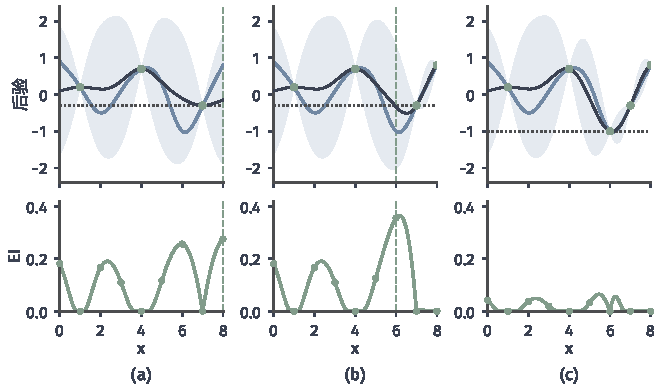
\includegraphics[width=112mm]{figures/05-optimization/05-stochastic-optimization/matplotlib/bo-rounds/figure.pdf}
 \caption{贯穿例的三轮选点。上行：蓝线是目标，深色线是后验均值，浅蓝带是均值上下两倍标准差，点线是当前最好值，绿点是读数。下行：绿线是EI，小点是整数候选上的分数。竖虚线是本轮选中的位置，依次为$x=8$、$x=6$、$x=0$。}
 \label{fig:bo-rounds}
\end{BookInlineFigure}

\subsection{初始设计}
\label{sec:bo-initial-design}

循环开始之前没有任何读数，采集函数没有依据（或者取决于先验，而先验下各处相同）。第一批点因此要在没有反馈的情况下放好，这一步称为\term{初始设计}（initial design）。本小节的问题是：放在哪里，放多少。

先验信息较少时，初始点的任务是覆盖搜索域的不同区域，同时为估计超参数提供不同间距的点对。图~\ref{fig:bo-initial-design}比较了单位方形上放九个点的三种办法。(a)均匀随机的点可能聚集，也可能在某些区域留白。(c)规则网格覆盖整齐，但投影到每个坐标上只有三个不同的值。(b)是\term{拉丁超立方抽样}（Latin hypercube sampling）：把每个坐标轴等分成九格，每行每列恰好放一个点，这样每个坐标轴的投影都分散。网格在高维时会失效，$n$维的$3^n$个格点很快超出预算。

\begin{BookInlineFigure}
 \centering
 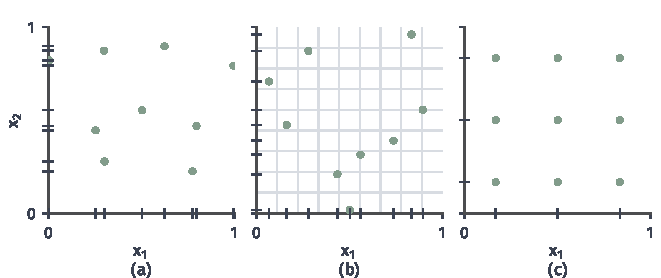
\includegraphics[width=112mm]{figures/05-optimization/05-stochastic-optimization/matplotlib/bo-initial-design/figure.pdf}
 \caption{单位方形上九个初始点的放置（固定随机种子）。(a)均匀随机；(b)拉丁超立方，浅灰线是九等分的格，每行每列恰好一个点；(c)规则网格。坐标轴上的短刻线是点在各坐标的投影，网格投影只有三个不同位置。}
 \label{fig:bo-initial-design}
\end{BookInlineFigure}

初始点不是越多越好，它们挤占后面的定向搜索。图~\ref{fig:bo-initial-budget}在贯穿例上固定总预算$T=8$，改变初始点数，其余用EI选点，统计$300$组随机初始点的平均终端误差。初始点不超过$4$时误差差别很小，因为这里的核是已知的，少量读数已经够用；初始点数达到$7$、$8$时，几乎没有定向评价的机会，平均误差升到$0.085$和$0.241$。

\begin{BookInlineFigure}
 \centering
 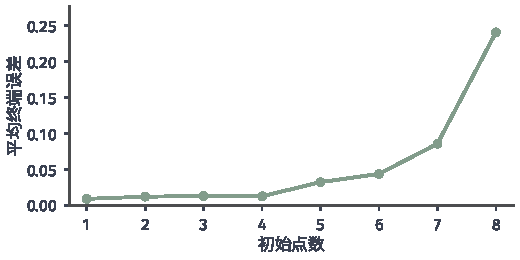
\includegraphics[width=88mm]{figures/05-optimization/05-stochastic-optimization/matplotlib/bo-initial-budget/figure.pdf}
 \caption{初始点数与最终效果。贯穿例，总预算$T=8$，初始点在$0.1$网格上均匀随机选取，其余用EI选点，纵轴是$300$组随机种子下的平均终端误差。初始点数等于$8$时全部预算都用于无反馈的覆盖。}
 \label{fig:bo-initial-budget}
\end{BookInlineFigure}

这个例子的核已知，所以很少的初始点就够了。核的超参数需要估计时，初始点太少会使边缘似然不可靠，代理在开始几轮可能严重失真，常见的经验是取搜索维数的若干倍（如$10n$），但这只是经验，总预算很小时要相应减少。

\subsection{采集函数求解}
\label{sec:bo-inner}

每轮要解一个内层优化问题：
\begin{equation}
 \bm{x}_{t+1}\in\argmax_{\bm{x}\in\bm{C}}\alpha_t(\bm{x}).
 \label{eq:bo-inner}
\end{equation}
它与外层目标的代价完全不同：$\alpha_t$是一个有解析式、可以快速求值的函数。但它一般不是凹函数，而且常有多个峰，本小节的问题就是怎样可靠地求它的最大点。

\paragraph{可用的导数}
真实目标不提供导数，但采集函数的导数完全来自代理。由式~\eqref{eq:bo-ei-derivatives}和链式法则，在$s_t(\bm{x})>0$的位置，
\begin{equation}
 \nabla\mathrm{EI}_t(\bm{x})=-\Phi(z)\nabla m_t(\bm{x})+\phi(z)\nabla s_t(\bm{x}).
 \label{eq:bo-ei-gradient}
\end{equation}
由式~\eqref{eq:bo-post-mean}和式~\eqref{eq:bo-post-cov}，令$\nabla\bm{k}_t(\bm{x})$表示$\bm{k}_t$对$\bm{x}$的Jacobi矩阵，并设核满足$k(\bm{x},\bm{x})$为常数，
\begin{align}
 \nabla m_t(\bm{x})&=\nabla\bm{k}_t(\bm{x})^\top\bm{A}_t^{-1}(\bm{y}_t-\bm{m}_{0,t})+\nabla m_0(\bm{x}),
 \label{eq:bo-grad-m}\\
 \nabla s_t(\bm{x})&=-\frac{\nabla\bm{k}_t(\bm{x})^\top\bm{A}_t^{-1}\bm{k}_t(\bm{x})}{s_t(\bm{x})}.
 \label{eq:bo-grad-s}
\end{align}
这些导数只要求核可导，不要求目标$f$可导。

用只有一个读数$F(7)=-0.3$的情形验算一下。取$x=6$，$b=-0.3$，则
\[
 k(6,7)=\tfrac12,\qquad \frac{\mathrm{d}k}{\mathrm{d}x}=-2\ln2\,(x-7)\,k\approx0.693.
\]
后验均值与方差及其导数是
\[
 m=-0.15,\quad m'\approx-0.208,\quad s\approx0.866,\quad s'\approx-0.400,
\]
其中$s'$由$(s^2)'=-2kk'$算得。这里$z\approx-0.173$，$\Phi(z)\approx0.431$，$\phi(z)\approx0.393$，代入式~\eqref{eq:bo-ei-gradient}，
\[
 \frac{\mathrm{d}\mathrm{EI}}{\mathrm{d}x}\approx0.431\times0.208-0.393\times0.400\approx-0.067.
\]
导数为负，说明从$x=6$向$x=7$走时，方差减小的损失超过了均值降低的收益。

\paragraph{多起点、候选筛选与随机搜索}
一个起点的局部上升只能到达它所在的峰。常用的做法是多起点局部优化：取一批起点，通常先在大量候选上计算$\alpha_t$，挑其中分数高的作起点，再用带约束的拟牛顿法作局部上升。也可以直接在候选集上比较分数，或用第~\ref{chap:random-search}章的随机搜索方法。这些方法都只求一个便宜函数的最大值，不增加昂贵评价。

图~\ref{fig:bo-inner-multistart}是贯穿例$t=5$时的情形。八个等距起点沿EI爬升，到达了四个不同的局部最大点，取值约为$0.042,0.049,0.065,0.057$，全局最大点在$x\approx5.46$。起点$x=7.5$附近EI几乎为零，梯度也几乎为零，上升根本走不动，这是平坦区域的常见困难，通常的对策是对EI取对数后再优化。

\begin{BookInlineFigure}
 \centering
 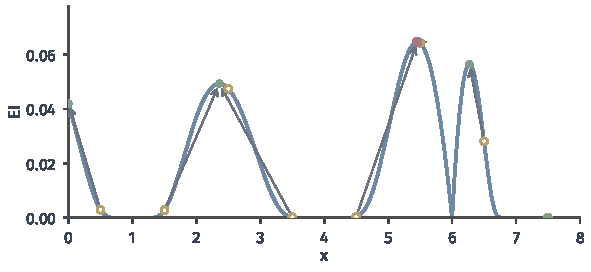
\includegraphics[width=100mm]{figures/05-optimization/05-stochastic-optimization/matplotlib/bo-inner-multistart/figure.pdf}
 \caption{内层问题的多起点求解。贯穿例$t=5$，蓝线是EI，黄色空心点是八个起点，灰色箭头是数值上升的起止，绿点是到达的局部最大点，红点是其中最好的点$x\approx5.46$。}
 \label{fig:bo-inner-multistart}
\end{BookInlineFigure}

对比这一轮的正文计算，整数候选集上的最大值是$\mathrm{EI}_5(0)\approx0.042$，而连续域上的最大点在$x\approx5.46$，取值$0.065$。内层问题的解法确实会改变外层的选点，这说明内层近似不是无关紧要的细节。内层近似求解也不自动得到采集函数的全局最优点；若分析某种算法的性质时假设了内层精确求解，实际运行时这个假设需要另外检查。

\subsection{观测更新}
\label{sec:bo-observation-update}

选定位置并运行真实评价之后，要回答的问题是：新读数应当怎样进入模型。

把新读数和它的噪声信息加入$\mathcal{D}_t$后，式~\eqref{eq:bo-update-mean}、式~\eqref{eq:bo-update-cov}更新候选点上的后验。若在搜索域的任意点上重新计算，需要更新Cholesky分解，也可以增量进行。设$\bm{A}_t=\bm{L}_t\bm{L}_t^\top$，新矩阵的因子只在末尾加一行：
\begin{equation}
 \bm{L}_{t+1}=\begin{bmatrix}\bm{L}_t&\bm{0}\\\bm{\ell}^\top&d\end{bmatrix},
 \label{eq:bo-chol-update}
\end{equation}
其中
\[
 \bm{\ell}=\bm{L}_t^{-1}\bm{k}_t(\bm{x}^+),\qquad
 d^2=k(\bm{x}^+,\bm{x}^+)+\tau^2-\bm{\ell}^\top\bm{\ell}.
\]
求$\bm{\ell}$只需一次前代，所以这一步需要$O(t^2)$次运算，不必花$O(t^3)$次重新分解。$d^2$恰好是新读数的预测方差$v$。如果这一轮重新估计了超参数，核矩阵整体改变，增量更新就不再适用，要重新分解。

这里要保留完整的历史，而不是只记住当前最好值。只记$b_t$的做法在第一轮之后只知道“最好值仍是$-0.3$”，看不到$x=8$的读数，也算不出$\mathrm{EI}_4(6)$从$0.257$升到$0.356$这个变化。未获改进的观测也有信息，它改变相关区域的预测，进而改变后续查询的价值。第一轮的$x=8$正是这种情形，图~\ref{fig:bo-rounds}(a)到(b)的变化说明了它的作用。
